\setlength{\parindent}{2ex}
\begin{chapter}{Introduction}\label{chapter:introduction}
  In addition to being a rich source of artistic and creative inspiration, pictures, or more precicely visual data, have been a crucial source of scientific information.
  Even the word ``observation'' generally connotes close visual scrutiny, and its use as a catch-all for the measured verification of a hypothesis exemplifies the central role of visual perception in science.
  Many important scientific results have used visual data to discover and explain natural phenomena; for example, visual observations such as the color and shape of various plant organs in Gregor Mendel's famous experiments on hybridized peas formed the primary source of data for developing his famous model for genetic inheritance \citep{magner2002}.
  Arthur Eddington's famous celestial observations in the early 20th century, which provided the first experimental evidence supporting Albert Einstein's general theory of relativity, recorded the gravitationally lensed path of a comet on photographs taken during a solar eclipse \citep{eddington1920}.
%  The richness of the raw data content in an image and our human propensity to digest visual information -- the focus of our mind's eye, so to say -- make visual data in images a compelling source of scientific evidence and information.
  Yet, in these cases, only the \emph{qualitative} components of the visual response and their relationship to the experiment were relevant.
  With the advent of the camera, photosensitive chemistry, and later digital imaging technology, high-fidelity recording of visual observations became possible, allowing the potential to \emph{quantitatively} analyze visual information.
  The ever-progressing technology in optical science and engineering are rapidly increasing the amount of data that can be measured in an image; yet, the extreme quantity and spatial organization that comes with high resolution data makes a rigorous quantitative analysis challenging.

  Images, when viewed quantitatively, can be described as the response of the incidence of light, and the subsequent exchange of energy, on a grid of regularly spaced grid elements, which we refer to as pixels.
  In our application, the grid elements are square.
  The domain of interest for imaging systems can vary greatly in both spatial dimension and the spectrum of light captured. 
  The energy response of light is spectrum dependent, and typically is analyzed at fixed bands of frequency with very high spatial resolution.
%  The raw volume of recorded data is usually very large.
  For example, astronomical images captured by the interstellar robotic probes Voyagers I and II measured 5 spectral bands in the visible spetrum on a pixel grid with dimension $800 \times 800$ \citep{voyager}.
  In medical imaging, computed tomography (CT) is an imaging process where a series of axial measurements of attenuation of electromagnetic radiation are used to reconstruct a cross-section of a scanned object \citep{epstein2008}.
  Of primary focus in this work are pulsed X-ray measurements, referred to as radiographs, that are used as an experimental diagnostic of high-energy physics experiments.  
  In this case, X-rays are pulsed through an experiment, then the attenuated X-rays excite a crystal that responds by luminescing visible light at an intensity related directly to the energy of the attenuated wave-front.  
  The light is then measured on a high resolution array (on the order of $1000\times1000$ or more) of carge coupled devices (CCD) calibrated to count photons at a specified spectral band.

  We have established the form that image data usually takes -- \emph{what} the data is. 
  Now, \emph{how} does one analyze it?
  Although images often provide a large volume of data, their spatial nature make measurements at each pixel highly dependent on measurments of adjacent pixels.
  A quantitative analysis of the image cannot assume that measured values are independent.
  But it is precisely this lack of independence that makes an image interesting -- independent image data is ``gray noise'' from which one can only infer the average of the measured pixels.
  %A quantitative analysis of image data must take into account pixel-to-pixel dependence.
  %That is, the measured values at one pixel depends heavily on adjacent or neighboring pixels, thus, one expects the measured data to be highly correlated.
  From a statistical point of view, the field of spatial statistics considers broadly the analysis of data that is structured and spatially correlated in this way.
%  The relatively recent date of this publication (in mathematical terms) coupled with the prevalence of image data prior to this, hints that the requisite tools for a rigorous statistical analysis require modern mathematical theory and state of the art computation.
  This field has had much development over the past half-century and has inspired a wealth of theory and computational tools, but is far from complete.
  Moreover, a broad field of scientific disciplines have considered image data, or more generally spatially correlated data, in one way or another; fields such as astronomy, astrophysics, biology, medicine, geology, computer science, and nuclear physics to name a few.
  The book \citep{cressie1993statistics} provides an excellent overview of the history and current methods for statistical methods for spatial data.
%  Each have a unique perspective on the problem, and a vast literature on the subject has accumulated.
  Although much work has been done, it is still a very active research area and is far from the level of consensus and understanding that analysis of independently sampled data has achieved. 
  The aim of this work is to develop and adapt current models and methods for estimation and quantifying uncertainty to a small component of image analysis related specifically to the \emph{system for capturing images}.
  Understanding this component is an important preliminary step to developing methods for quantitatively analyzing the images themselves.

\section{Modeling blur with a PSF}
  
  One major component of the spatial relationship of neighboring pixels of an image is due to blur from the imaging instrumentation.
  That is, under the assumption that arbitrary images are consistently measured by the modeled system, what contribution does this system have on how pixels are related, and how can we quantify this relationship?
  A widely used model for blurring \citep{hansen2010,jain1989,vogel2002,epstein2008} expresses this relationship as a linear filter that maps the ideal image $f$ to $b$ by integrating
  %this relationship through a point-wise integral product with a function that describes interaction with neighboring points, e.g.
\begin{equation}\label{eq:generalFilterForm}
  b(x,y) = \iint_{\RR^2} \kappa(x,y;s,t) f(s,t)\,dsdt
\end{equation}
  where $b(x,y)$ represents the intensity of the blurred image at $(x,y)$; $f(s,t)$ represents the intensity of the ideal un-blurred image at $(s,t)$; and $\kappa$ is the kernel of the filter, which characterizes the blurring process.
  Informally, we can view the effect of blur point-wise by taking $f(s,t)$ as a point light source located at $(\bar x,\bar y)$, then $b(\bar x,\bar y) = \kappa(x,y;\bar x,\bar y)$ represents the ``spread'' at the point source.
%  The form of $\kappa$ is guided by optical principles and the physics of the system which generally dictate that at each $(x,y)$ the function that maps $(s,t)$ to $\kappa(x,y;s,t)$ is concentrated (in the measured or integrated sense) at $(x,y)$ and continuously decays as the distance from $(s,t)$ to $(x,y)$ increases.
%  The function in \eqref{eq:generalPsf} is often interpreted as a family of PSFs $\kappa(x,y;\cdot,\cdot)$ indexed at each $(x,y)$.
  When $f$ and $g$ are elements of $L^p$ spaces and the effect of blur is spatially invariant (that is, invariant to translation), then the filter can be expressed through convolution with some $k$ \citep{grafakos2014}, so \eqref{eq:generalFilterForm} reduces to
\begin{equation}\label{eq:deconvolutionProblem}
  b(x,y) = \iint_{\RR^2} k(x-s,y-t) f(s,t)\,dsdt.
\end{equation}
  The function $k$ is referred to as the \emph{point spread function} (PSF) of the system.
  The assumptions for modeling blur in this form are quite common, and methods that estimate $f$ given $b$ and $k$ are referred to as deconvolution techniques.
  Note that a change of variables by $s'=x-s$ and $t'=y-t$ results in a convolution of $k$ by $f$, which is to say that convolution, as an operation, is symmetric.
  That is
\begin{equation}\label{eq:dualConvolutionDeterministic}
  b(x,y) = \iint_{\RR^2} k(s,t) f(x-s,y-t)\,dsdt.
\end{equation}
  This dual relationship between the PSF and the image will allow us to use the framework and many of the tools of deconvolution for the problem of PSF estimation.

  Typically, deconvolution methods assume that the form of the PSF can be accurately described by modeling the imaging system \citep{jain1989,hansen2010}, but for complex imaging systems such as the one described for X-ray radiography, this is not realistic.
  Instead, if the imaging system is designed so that repeated images can be taken under consistent conditions, then by convolution symmetry in \eqref{eq:dualConvolutionDeterministic}, the blurring of a \emph{known calibration image} can be cast as deconvolving the PSF from the ideal $f$ corresponding to the known image.

  Recall that the PSF models the blurring response of a single point.
  So, a direct estimate of $k$ can be obtained by imaging a bright point source, which approximates the impulse response to \eqref{eq:dualConvolutionDeterministic}.
  In astronomical imaging, the point source can be a bright distant star, or in a controlled setting where visible light is measured, a focused laser beam provides a good point source estimate.
  However, in the spectral regime of high-frequency X-rays, the problem of focusing high frequency-light is notoriously difficult and usually is impractical in situations of interest, so a point source estimate of the PSF is usually unavailable at these frequencies.
  Instead, the system response of a uniformly opaque calibration object with a simple geometry can be measured.
  Under the assumption that the object is sufficiently thick so that X-rays are completely attenuated on the profile of the object, then $f$ is given by an indicator function $E \subseteq \RR^2$ determined by the object's profile.
  Calibration objects typically have simple geometry and reduce the complexity of solving the deconvolution problem \eqref{eq:dualConvolutionDeterministic}.  
  For example, the object could be a circular aperture or two perpendicular edges aligned with the imaging plane \citep{doering1992,watson1993}.
  An additional assumption of \emph{radial symmetry} on $k$, will allow for a very simple calibration object -- an edge. 
  That is, if the calibration object completely attenuates X-rays along a vertical edge at a fixed location in the imaging plane, then $E=\{(s,t):s\ge0\}$ and $f(s,t) = f_E(s,t) = 1$ if $s\ge0$ and $0$ if $s <0$. 
  See \Cref{fig:edgePicture} for a schematic of the calibration object and measurement system and \Cref{fig:edgeData} for an example of recorded intensity data.
  The model for blur in \eqref{eq:dualConvolutionDeterministic} reduces to
\begin{equation}\label{eq:psfForwardModelDeterministic2D}
  b(x,y) = \iint_{\RR^2} k(s,t) f_E(x-s,t)dsdt. 
\end{equation}
  Note that $b$ does not depend on $y$, and $f_E$ does not depend on $t$, so denoting $b(x,0) = b(x)$ and $f_E(x-s)=f_E(x-s,0)$, \eqref{eq:psfForwardModelDeterministic2D} reduces to
\begin{equation}\label{eq:psfForwardModelDeterministic}
  b(x) = \iint_{\RR^2} k(s,t) f_E(x-s)dsdt. 
\end{equation} 
  The integral equation in \eqref{eq:psfForwardModelDeterministic} models the problem of estimating a PSF from the image of an edge, and finding a solution to this problem is the primary focus of this work.

  In general, estimating $k$ from $b$ in \eqref{eq:psfForwardModelDeterministic} is underdetermined, since there are generally many distinct $k$ that can result in the same output $b$.
  To see this, note that 
  \begin{equation}
    \int_{-\infty}^{\infty} te^{-t^2 - s^2}dt = 0
  \end{equation}
  for all $s$ since the integrand is odd in $t$.
  So given any solution $k$, $k(s,t)+te^{-t^2 - s^2}$ is also a solution but is \emph{not} radially symmetric.
  The form of \eqref{eq:psfForwardModelDeterministic} is not immediately useful for analyzing the problem, and in the next sections, we will transform variables in \eqref{eq:psfForwardModelDeterministic} in two different ways that will show that the PSF estimation problem fits within the broad category of mathematical study known as \emph{inverse problems}.
  
\section{The Abel transform and a deterministic solution}
  In this section we show that radial symmetry is sufficient to guarantee a unique analytic answer.
  This will lay out an analytic solution to \eqref{eq:psfForwardModelDeterministic}. 
  However, it will be inadequate as we will see in the following section.

  A large part of designing a system for imaging is to minimize the effect of blur.
  Often, limitations due to physical laws put a lower bound on the measurement precision so that even an optimal design cannot ignore the effect of blur.
  Although arbitrary resolution may be impossible, engineering effort can still optimize accuracy, or, equivalently, minimize bias.
  Hence, an optimally designed imaging system should exhibit isotropic blur (an absence of direction bias), so that, in the convolution model, the PSF is radially symmetric.
  In fact, many parametrically modeled PSFs assume radially symmetry \citep{doering1992,jain1989,kundur1996blind,watson1993}.  

  When one assumes that the PSF of their system is radially symmetric, then it has a unique one-dimensional representation.
  That is, there exists a function $p$ defined on $[0,\infty)$ so that $k(s,t) = p\left(\sqrt{s^2 + t^2}\right)$.  
  The function $p$ is referred to as the radial profile of $k$.
  Substituting $p$ and viewing \eqref{eq:psfForwardModelDeterministic} as iterated integration, the inner integral has the form
  \begin{equation} \label{eq:abelTransform}
    \ell(s) \eqdef \int_{-\infty}^\infty p\left(\sqrt{s^2 + t^2}\right)\,dt
  \end{equation}
  The function $\ell(s)$ is the integration along a line perpendicular to the edge $E$, and its form is commonly encountered in other imaging applications with radial geometry, such as tomographic imaging science.
  The transformation that takes $p$ to $\ell$ is known as the \emph{Abel transform}, and for its study in imaging science, see \citep{bracewell,epstein2008,knill93}.
  Substituting into \eqref{eq:psfForwardModelDeterministic} gives
  \begin{align}
    b(x) &= \int_{-\infty}^x \left(\int_{-\infty}^\infty p\left(\sqrt{s^2 + t^2}\right)\,dt\right)ds \nonumber \\
         &= \int_{-\infty}^x \ell(s)ds. \label{eq:abelForward}
  \end{align}

  Observe that $b$ exhibits point symmetry about $b(0)$.
  To see this analytically, for $x>0$ the formulation in terms of the Abel transform in \eqref{eq:abelForward} gives
  \begin{align}
    b(x) &= \int_{-\infty}^0 \ell(s)ds + \int_0^x \ell(s)ds \nonumber \\
         &= b(0) - \int_0^{-x}\ell(s')ds'  \nonumber \\
         &= b(0) - b(-x).
  \end{align}
  Hence, data defined on either $x\in(-\infty,0]$ or $x\in[0,\infty)$ should be sufficient for estimating $p$.

%  The collection of line integrals parametrized by their angle of incidence is called the Radon transform of $k$, and when $k$ is radially symmetric, the transform is completely determined by a single projection.
%  The operator that takes the radial profile $p$ to $l$ is called the Abel transform and is encountered in tomographic imaging.
  The Abel transform has an explicit expression for its inverse given by
  \begin{equation} \label{eq:inverseAbel}
    p(r) = -\frac{1}{\pi r} \frac{d}{dr}\left(\int_r^\infty \frac{\ell(s) s ds}{ (s^2 - r^2)^{1/2} } \right).  
  \end{equation} 
  The following calculations verify \eqref{eq:inverseAbel}.

  \begin{prop}
    Suppose that $p(r)$ is such $\lim_{r\to\infty}p(r) = 0$ and $\ell(s)$ in \eqref{eq:abelTransform} is point-wise defined and the integral in \eqref{eq:inverseAbel} is finite for each $r$, then equation \eqref{eq:inverseAbel} holds.
  \end{prop}
  \begin{proof}
  We can express the inner integral in \eqref{eq:abelForward} as
  \begin{equation}
    \ell(s) = 2\int_{|s|}^\infty \frac{p(t) t}{(t^2 - s^2)^{1/2}}\,dt \label{eq:abelForward2}
  \end{equation}
  by symmetry of the integrand (it is even) and a change of variable by $r = s^2 + t^2$.
  Now, interchanging the order of integration in \eqref{eq:inverseAbel} results in
  \begin{align} 
    \left(\int_r^\infty \frac{\ell(s) s ds}{ (s^2 - r^2)^{1/2} } \right)  
    &= \int_r^\infty\int_s^\infty \frac{p(t) ts}{(s^2 - r^2)^{1/2}(t^2 - s^2)^{1/2}}\,dtds \nonumber\\
    &= \int_r^\infty p(t) t\int_r^t \frac{s}{(s^2 - r^2)^{1/2}(t^2 - s^2)^{1/2}}\,dsdt. \label{eq:inverseAbelderive1}
  \end{align} 
  Another change of variables by $s^2 = \tau t^2 + (1-\tau)r^2$ (note $s\ge0$)
 % , results in $2sds = (t^2 - r^2)d\tau$, 
  so that the inner integral in \eqref{eq:inverseAbelderive1} is
  \begin{equation}
    \int_r^t \frac{s}{(s^2 - r^2)^{1/2}(t^2 - s^2)^{1/2}}\,ds
    = \frac 12 \int_0^1 \frac {1}{\tau^{1/2}(1-\tau)^{1/2}}\,d\tau. \label{eq:gammaIntegral}
  \end{equation}
  Note that the resulting integral is independent of both $r$ and $t$, thus, is constant. To evaluate it, recall the Gamma function identity
  \begin{equation} 
    \frac{\Gamma(\alpha)\Gamma(\beta)}{\Gamma(\alpha + \beta)} = \int_0^1 \tau^{-\alpha}(1-\tau)^{\alpha -1}\,d\tau,
  \end{equation}
  from which the expression in \eqref{eq:gammaIntegral} reduces to $\pi/2$.
  Collecting these results and applying the fundamental theorem of calculus with the assumption that $\lim_{r\to\infty}p(r) = 0$, proves the identity in \eqref{eq:inverseAbel}.
\end{proof}
  
  With this result, $p$ can be analytically recovered from $b$ in \eqref{eq:abelForward}. 
  That is, given $b(x)$, the fundamental theorem of calculus gives $\ell(s)$ by differentiating $b(x)$, then applying the inversion formula in \eqref{eq:inverseAbel} to $b'(x)$ gives the radial profile $p(r)$.
  Hence, the assumption of radial symmetry sufficiently constrains the problem to uniquely determine the PSF from an edge calibration object illustrated in \Cref{fig:edgeData}.

  In theory, we have outlined a solution to the problem, but there is one more component to the noise-free model that has not been addressed -- random effects due to measurement error -- for which a direct application of outlined method on measured data will fail spectacularly, due to the estimation problem being ``ill-posed'' which we address in the next section.

\section{PSF reconstruction as an ill-posed inverse problem}
  
The analytic solution outlined in the last section will not be sufficient when measurement errors are introduced, and the subtlety lies in evaluating the derivatives in \eqref{eq:inverseAbel} and \eqref{eq:abelForward}.
In this section, we will return to \eqref{eq:psfForwardModelDeterministic}, and perform a different variable transformation to explicitly illustrate the difficulty of measurement error, and in doing so, will derive a form that is more suitable for numerical discretization.

  The measurements of the imaging system are generally not deterministic and are subject to measurement noise.
  Precisely modeling the stochastic effect of measurement error is system dependent and can be quite complicated.
  In the X-ray radiography example, uncertainty can enter into the system at the luminescing crystal response, at the counts of CCD array, or through the electrical transmission of the signal.
  In order to be broadly applicable, and appealing generally to various central-limit-theorem-like results in probability \citep{durrett2010probability}, we model the stochastic measurement effect in aggregate as an additive, independent Gaussian noise process with zero mean and unknown variance.  
  For now, this assumption can be viewed as a small perturbation from the model, but its form will be important for the inference techniques developed in subsequent chapters.
  %The complete description of the model from which the PSF will be estimated is
  %  \begin{equation}\label{eq:psfForwardModelStochastic} 
  %    b(x) = \iint_{\Omega} k(s,t) f(x-s)dsdt + \eps_x  
  %  \end{equation}
  %where each $\eps_x \sim N(0,\sigma^2)$ and independently (in $x$) for some unknown variance $\sigma^2$.  

  Estimating a quantity of interest, in our case $k$, from indirect and noisy measurements, $b$, with a model where an operator takes $k$ \emph{to} $b$ (referred to as the \emph{forward operator}) is called an inverse problem.  
  The problem is called well-posed when the forward operator is invertible, and the inversion is insensitive to small perturbations.
  These famous conditions were laid out by Jacques Hadamard in the early 20th century \citep{hadamard1902}, but a number of important applications have arisen (among those computational imaging) where these conditions are violated, enough to the extent that the term ``inverse problems'', as it refers to the mathematical research area, is exclusively devoted to solving these \emph{ill-posed} problems.
  In particular, most cases of interest %are when the measurement model results in data \emph{not} in the range of the model operator and 
  exhibit a model where the inverse of the forward operator is very sensitive to perturbations.

  The discussion thus far for PSF reconstruction has been somewhat informal, as we have not defined a space for the PSF or its radial representation, so we have not formally defined a model forward operator.
  Defining these spaces in detail is technical and will be addressed in in Chapter 2; however, assuming these spaces have been defined, we can illustrate that the problem of reconstructing the radial profile is ill-posed.

  Returning to \eqref{eq:psfForwardModelDeterministic}, a variable transformation
  %(again assuming $\Omega$ is full measure in $\RR^2$)  
  by $(s,t) = T(r,v) = (r\cos v,r\sin v)$, has $|dT(r,v)| = r$ and 
  \begin{align}
    b(x) &= \int_0^\infty p(r) \left( \int_{-\pi}^\pi f_E(x - r\cos v)dv \right)\,r dr\nonumber \\
         &= \int_0^\infty p(r) g(x,r) r dr, \label{eq:radialForwardModelDeterministic}
  \end{align}
where
\begin{equation} \label{eq:radialForwardKernel}
  g(x,r) \eqdef \left\{\begin{array}{lr}
    0 & x < - r\\
    2(\pi - \acos(x/r)) & |x| < r\\
    2\pi &  x> r
  \end{array}\right..  
\end{equation}
  To see that $g$ has this form, note that integrating $f_E(x-r\cos v)$ is the radian measure of the set $\{v\in(-\pi,\pi): r\cos v \le x\}$; see \Cref{fig:radialForwardKernel}.  

  There are three key observations to make.
  From this viewpoint, the forward model is now a one-dimensional integral equation on the radial profile as opposed to the two-dimensional problem in \eqref{eq:psfForwardModelDeterministic}.
  Second note that $g(x,r)$ is continuous (although it has a discontinuity in its partial derivatives across $r=s$).
  Finally, recall that the graph of $b(x)$ exhibits reflection symmetry about $b(0)$.
  So, $b(x)$ defined on either $(-\infty,0]$ or $[0,\infty)$ completely determines $p$.

  With these observations, we can define $G: \mathcal H_1 \to \mathcal H_2$ is an operator between closed isometric subspaces of $L^2([0,\infty))$ that acts by the integral equation in \eqref{eq:radialForwardModelDeterministic}, then $G$ is a compact Hilbert-Schmidt operator since $g$ is continuous and $\mathcal H_1$ and $\mathcal H_2$ are seperable Hilbert spaces.
  Thus, the spectral theory for such operators implies that $G$ is invertible, has a countable spectrum that has zero as a limit point, and hence, $G^{-1}$ is unbounded, which results in an ill-posed problem. 
  See one of many texts on functional analysis \citep{bachman1966,rudin1991} and \citep{tikhonov1963,vogel2002,morozov1993} for the analytic treatment of ill-posed problems.

  Solving ill-posed inverse problems requires \emph{regularization} of the unbounded inverse.
  Recall that the original formulation of the problem is cast in terms of deconvolution, and much of the literature of inverse problems is devoted to this subject.
  This work draws heavily from techniques for that purpose. 
  In particular, we will take a Bayesian approach to the inverse problem so that in addition to estimating $k$, uncertainties in the estimate can quantified by analysing the posterior distribution.
  These methods have been the subject of much recent research (see the books \citep{calvetti2007introduction,kaipo2005,stuart2010}), and the problem of PSF reconstruction fits neatly into that framework once the spaces $\mathcal H_1$ and $\mathcal H_2$ have been defined.

\begin{figure}
  \begin{center}
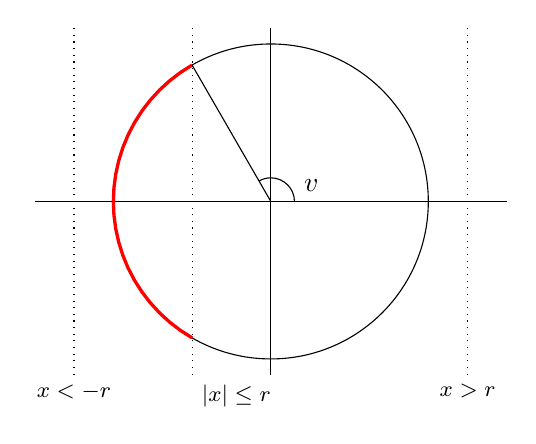
\begin{tikzpicture}
  \draw (0,-2.2) -- (0,2.2);
  \draw (-3,0) -- (3,0);
  \draw[dotted] (-2.5,-2.2) node[below]{\footnotesize$x<-r$} -- (-2.5,2.2);
  \draw[dotted] (2.5,-2.2) node[below]{\footnotesize$x>r$} -- (2.5,2.2);
  \draw[dotted] (-1,-2.2) node[below right]{\footnotesize$|x|\le r$} -- (-1,2.2);

  \draw (0,0) circle[radius=2];
  \draw[very thick,red,domain=120:240] plot ({2*cos(\x)},{2*sin(\x)});
  \draw (0,0) -- (-1,{sqrt(3)});
  \draw (.3,0) node[above right]{$v$} arc [radius=.3,start angle=0,end angle=120];
\end{tikzpicture}
  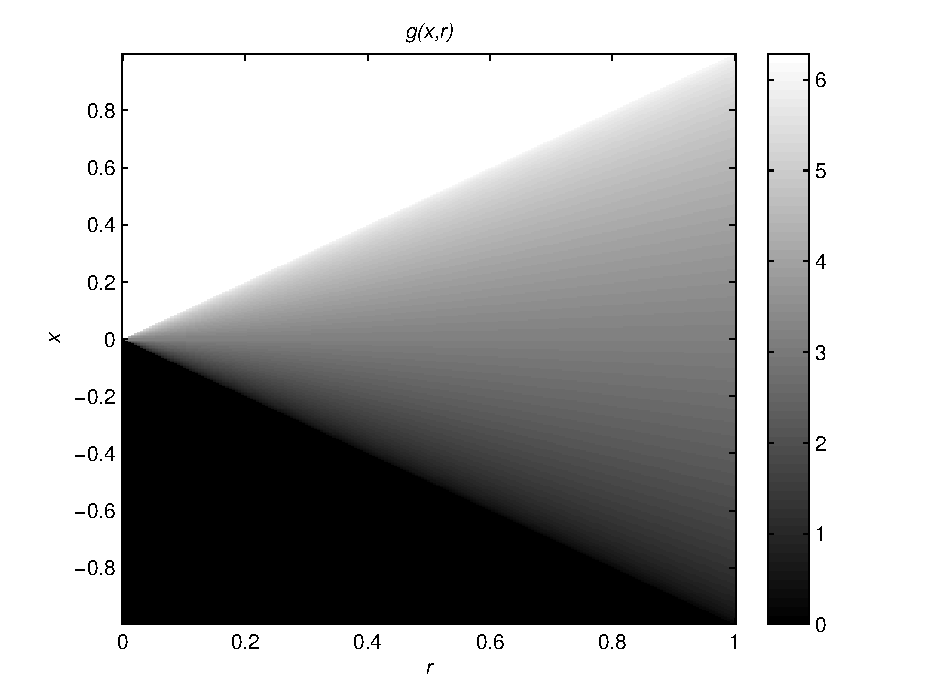
\includegraphics[width=.5\textwidth]{figures/g_function.pdf}
\end{center}
\caption{ The PSF forward integral operator kernel $g(x,r)$ represented as the arc measure of $v$ in $(-\pi,\pi)$ where $x \ge r\cos v$. }\label{fig:radialForwardKernel}
\end{figure}


\begin{figure}
  \begin{center}
    \begin{tikzpicture}[scale=.8,every node/.style={minimum size=1cm},on grid]
      \def\myxslant{0.1}
      \def\myyslant{-0.4}

	\begin{scope}[
		xshift=40,
		every node/.append style={
		xslant=\myxslant,yslant=\myyslant},xslant=\myxslant,yslant=\myyslant
	]
	\draw (0,0) rectangle (2.8,2.2);
%	\draw[fill=black] (1,0) rectangle (2.8,2.2);
	\end{scope}

	\begin{scope}[
		yshift=-20,
		every node/.append style={xslant=\myxslant,yslant=\myyslant},
		xslant=\myxslant,yslant=\myyslant
	]
	\draw[x=.314cm,y=.2cm,z=.2cm,thick,-latex,red] (0,0,0)
	  sin ++(0,1,1) cos ++(0,-1,1) sin ++(0,-1,1) cos ++(0,1,1)
	  sin ++(0,1,1) cos ++(0,-1,1) sin ++(0,-1,1) cos ++(0,1,1)
	  sin ++(0,1,1) cos ++(0,-1,1) sin ++(0,-1,1) cos ++(0,1,1);
	\draw[x=.314cm,y=.2cm,z=.2cm,thick,-latex,red] (-2,0,0)
	  sin ++(0,1,1) cos ++(0,-1,1) sin ++(0,-1,1) cos ++(0,1,1)
	  sin ++(0,1,1) cos ++(0,-1,1) sin ++(0,-1,1) cos ++(0,1,1)
	  sin ++(0,1,1) cos ++(0,-1,1) sin ++(0,-1,1) cos ++(0,1,1);
	\draw[x=.314cm,y=.2cm,z=.2cm,thick,-latex,red] (-4,0,0)
	  sin ++(0,1,1) cos ++(0,-1,1) sin ++(0,-1,1) cos ++(0,1,1)
	  sin ++(0,1,1) cos ++(0,-1,1) sin ++(0,-1,1) cos ++(0,1,1)
	  sin ++(0,1,1) cos ++(0,-1,1) sin ++(0,-1,1) cos ++(0,1,1);

	\pgfmathsetmacro{\cubex}{2}
	\pgfmathsetmacro{\cubey}{2.5}
	\pgfmathsetmacro{\cubez}{1}
	\draw[black,fill=gray,opacity=.75] (3.7,3,0) -- ++(-\cubex,0,0) -- ++(0,-\cubey,0) -- ++(\cubex,0,0) -- cycle;
	\draw[black,fill=gray,opacity=.75] (3.7,3,0) -- ++(0,0,-\cubez) -- ++(0,-\cubey,0) -- ++(0,0,\cubez) -- cycle;
	\draw[black,fill=gray,opacity=.75] (3.7,3,0) -- ++(-\cubex,0,0) -- ++(0,0,-\cubez) -- ++(\cubex,0,0) -- cycle;

	\draw[x=.314cm,y=.2cm,z=.2cm,thick,-latex,red] (4,0,0)
	  sin ++(0,1,1) cos ++(0,-1,1) sin ++(0,-1,1) cos ++(0,1,1)
	  sin ++(0,1,1) cos ++(0,-1,1) sin ++(0,-1,1) cos ++(0,1,1);
	\draw[x=.314cm,y=.2cm,z=.2cm,thick,-latex,red] (2,0,0)
	  sin ++(0,1,1) cos ++(0,-1,1) sin ++(0,-1,1) cos ++(0,1,1)
	  sin ++(0,1,1) cos ++(0,-1,1) sin ++(0,-1,1) cos ++(0,1,1);
	\end{scope}

	\begin{scope}[
		xshift=180,
		every node/.append style={xslant=\myxslant,yslant=\myyslant},
		xslant=\myxslant,yslant=\myyslant
	]
	    \draw (0,0) rectangle (2.8,2.2);
	    \tikzfading[name=fade left,left color = transparent!100,right color = transparent!0]
	    \draw[path fading=fade left,fading transform={rotate=-30},fill=black] (.9,0) rectangle (1,2.2);
	    \draw[fill=black] (1,0) rectangle (2.8,2.2);
	\end{scope}

	\begin{scope}[
		xshift=300,
		every node/.append style={xslant=\myxslant,yslant=\myyslant},
		xslant=\myxslant,yslant=\myyslant
		]
	    \draw (0,0) rectangle (2.8,2.2);
	    \tikzfading[name=fade left,left color = transparent!100,right color = transparent!0]
	    \draw[path fading=fade left,fading transform={rotate=-30},fill=black] (.9,0) rectangle (1,2.2);
	    \draw[fill=black] (1,0) rectangle (2.8,2.2);
	    \draw[step=1mm, black] (0,0) grid (2.8,2.2); %defining grids
	\end{scope}
	

    %    %putting arrows and labels:
	\node at (2,2.5) (label1) {Opaque Edge};
	\draw[-latex,thick] (2,-2) to node[below] {Image System Response} (7.5,-2);
	\node at (4.65,-3.4) (math1) {$\displaystyle{b(x)=\iint_{\RR^2} k(s,t) f(x-s)\,dsdt}$};

	\node at (7,2.5) (label3) {Blurred Profile};

	\node at (12,2.5) (label2) {Recorded Data};
	\draw[-latex,thick] (9,-2) to node[below]{Measurement error} (13.2,-2);
	\node at (11,-3.4) (math1) {$+\eps_x \sim N(0, \sigma^2)$};

    \end{tikzpicture}
  \caption{ A schematic of the measurement model for an X-Ray image of an edge. An opaque block aligned with the imaging plane blocks light on the half plane to produce a blurred edge.}\label{fig:edgePicture}
\end{center}
\end{figure}

\begin{figure}
\begin{center}
  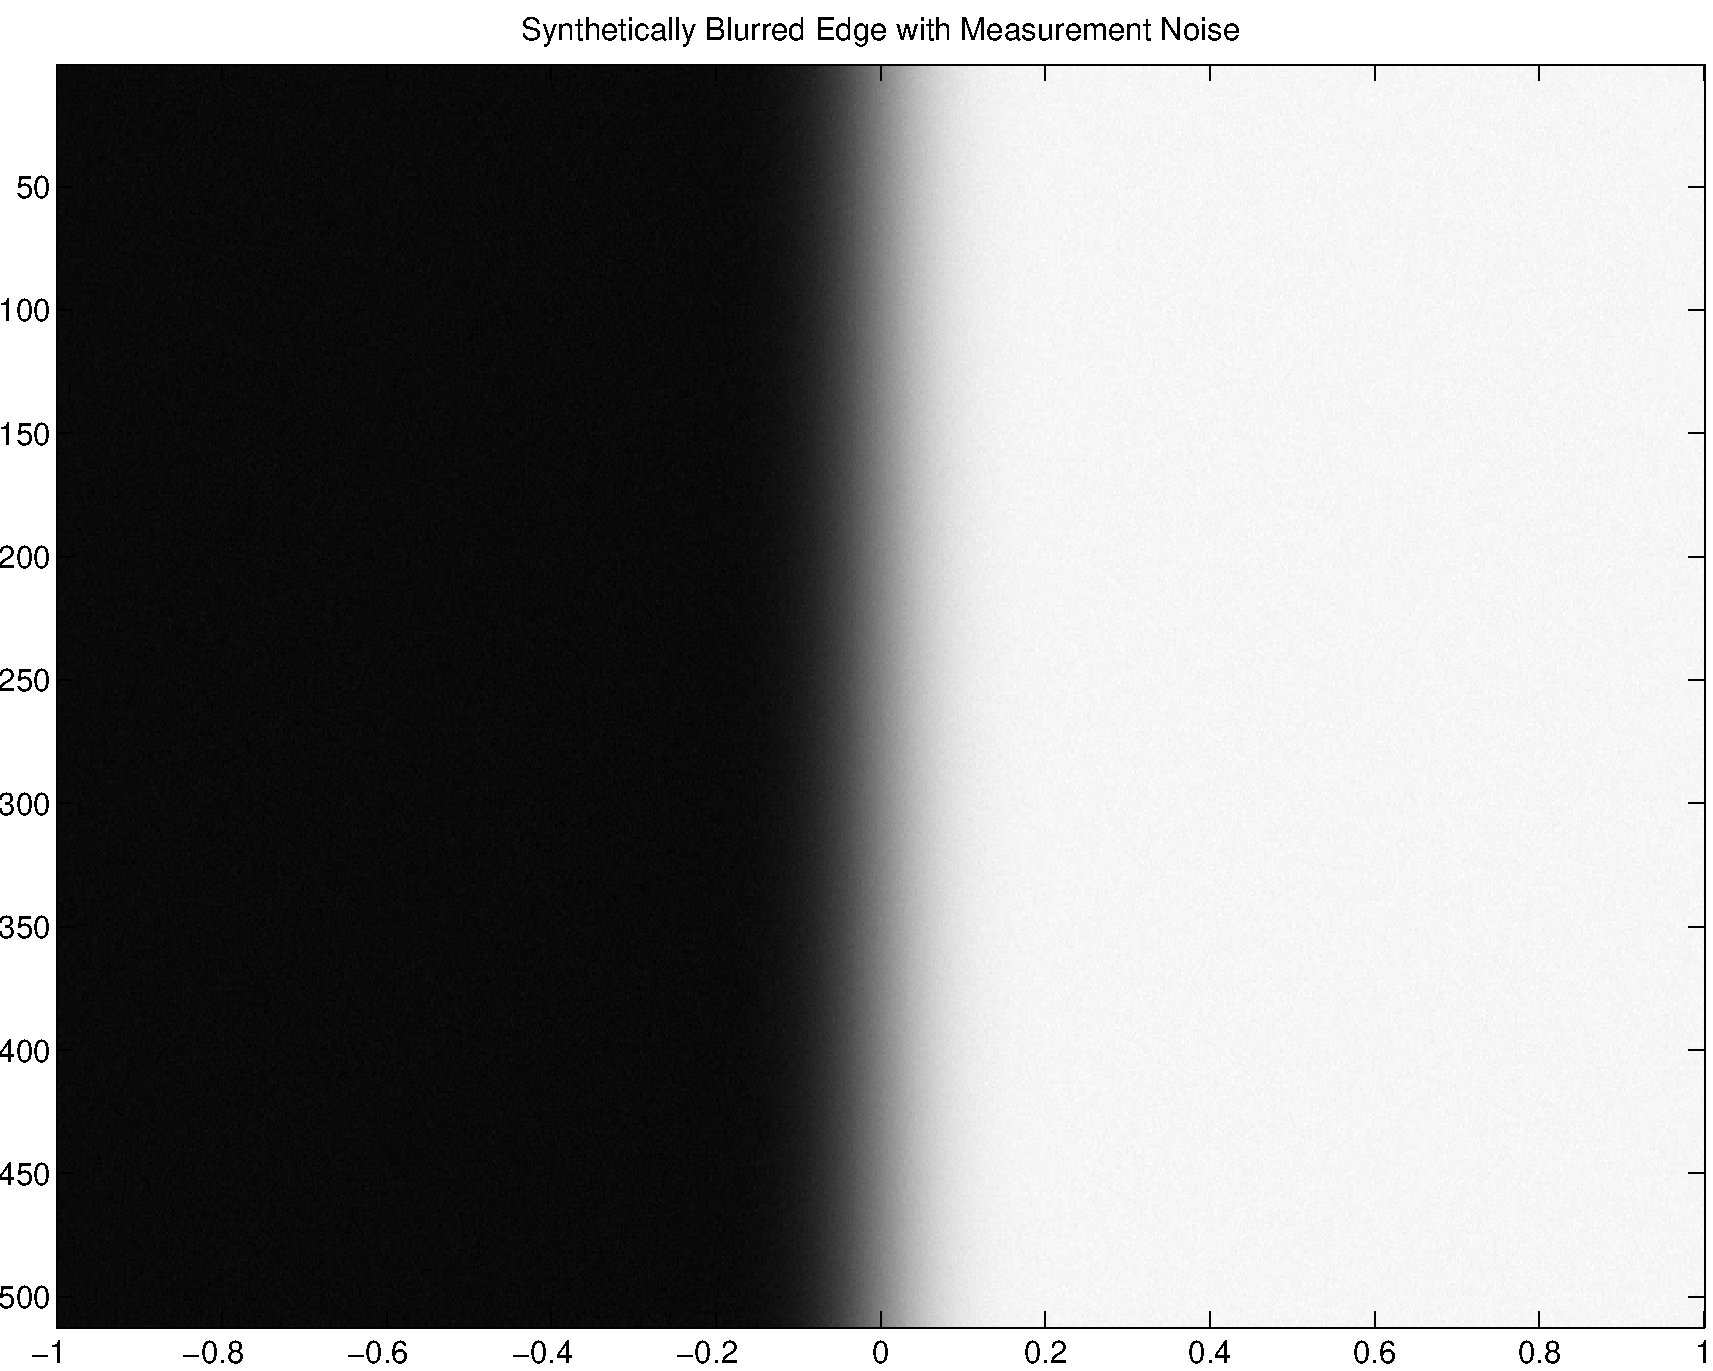
\includegraphics[width=.45\textwidth]{figures/blurredEdgeData.pdf}
  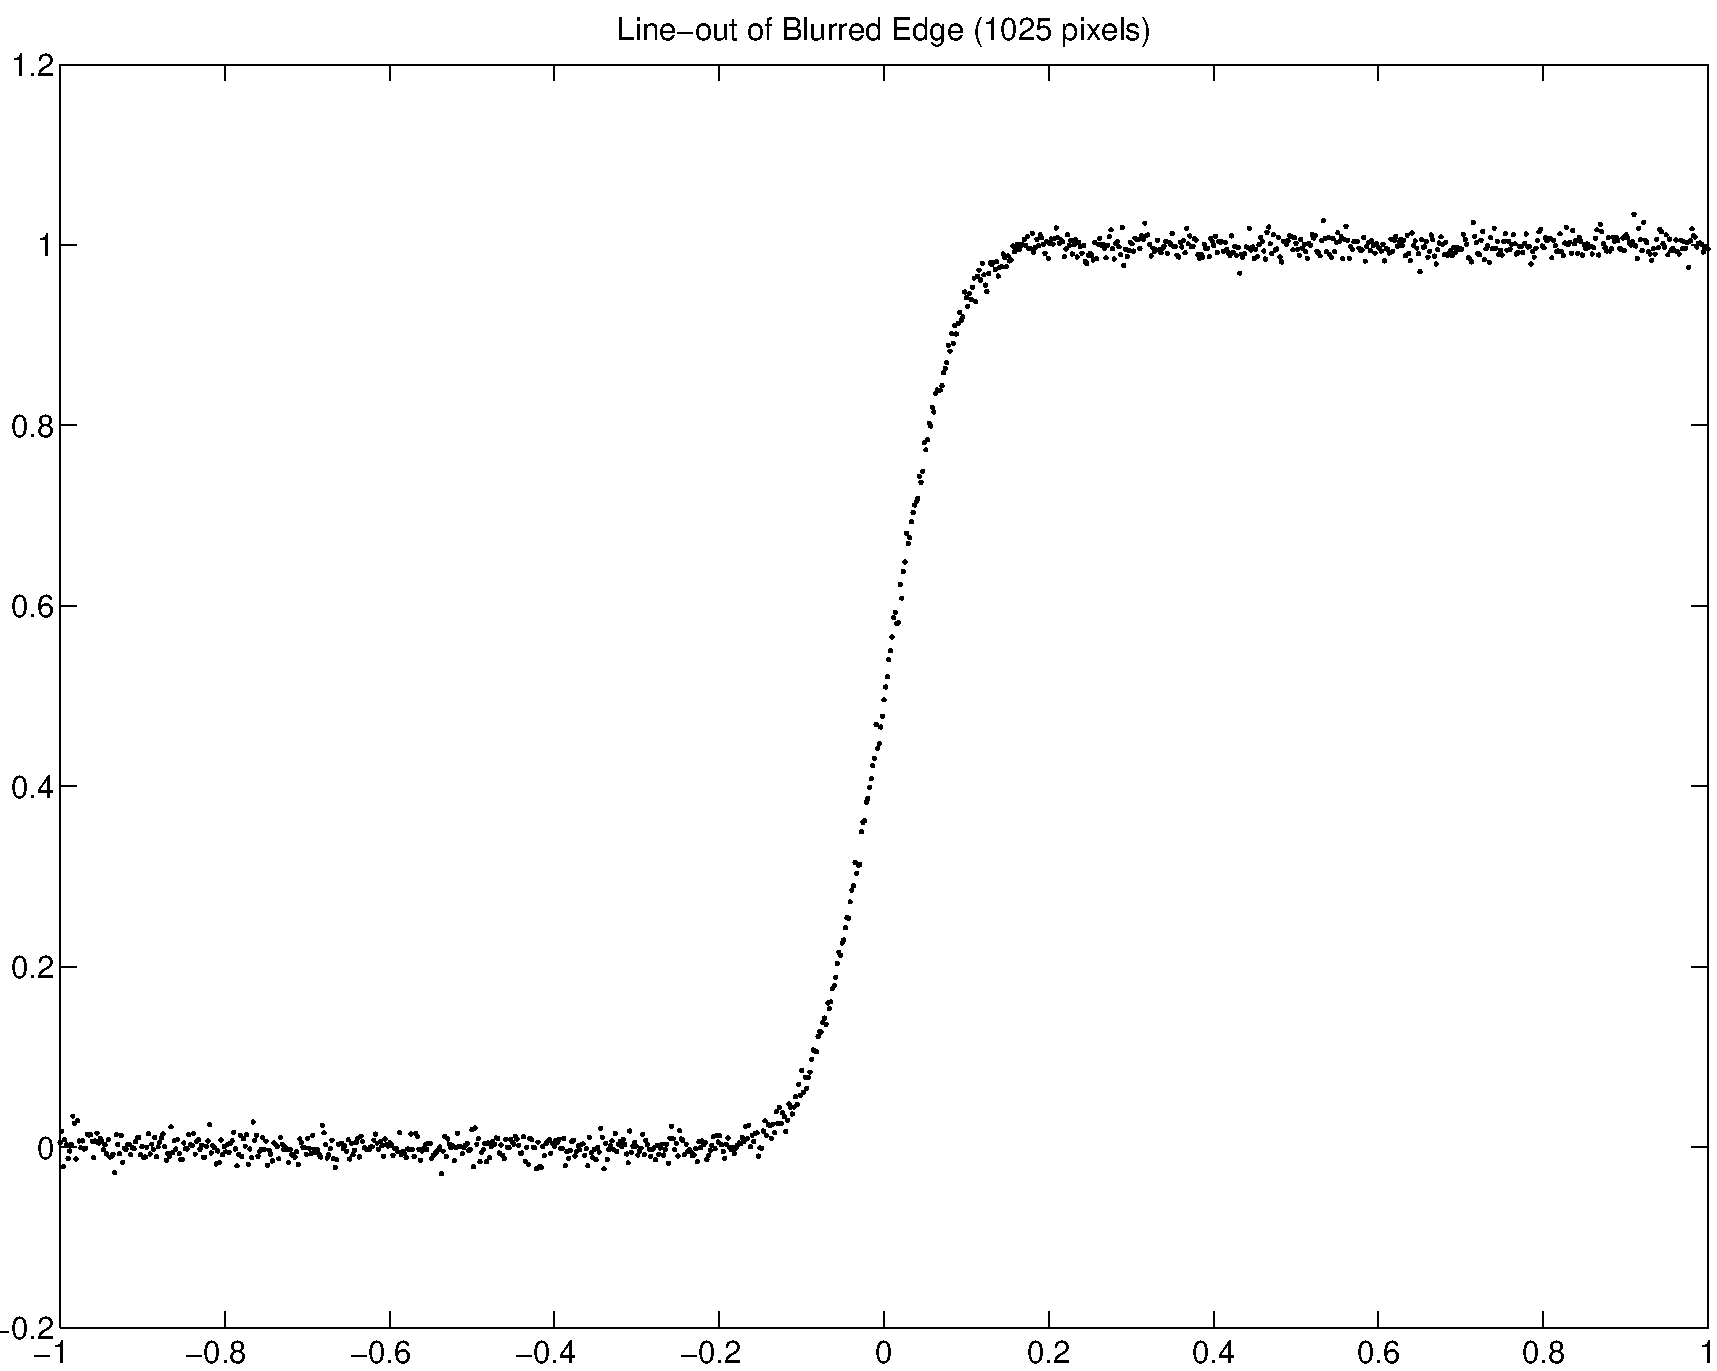
\includegraphics[width=.45\textwidth]{figures/psfLineoutData.pdf}
  \caption{A synthetically blurred edge with simulated measurement error and a line-out (horizontal cross-section) from the data.} \label{fig:edgeData}
\end{center}
\end{figure}

  
\section{Organization}
  In the next chapter, we will give a basic outline of Bayesian estimation techniques for the problem of PSF reconstruction.
  Primarily, we will develop the theoretical framework of how inference can be carried out on the radial profile of the PSF, when prior assumptions are placed on the PSF itself.
  Chapter 2 will be mainly theoretical, but the explicit forms for the discrete model of the forward operator and prior are motivated and derived there.
  Chapter 3 will give details on how to carry out the estimation on a computer.
  There, we will deal with how to discretely represent each of the necessary components in the estimation problem.
  We will also motivate and present the design of a detailed algorithm for carrying out the estimation outlined in Chapter 2.
  Finally, in Chapter 4, we present the results of an implementation on synthetically derived data and on measured data from a high-energy X-ray imaging system at the U.S.~Department of Energy's Nevada National Security Site.
  We will end with a discussion of conclusions and possible future work.


\end{chapter}
